\documentclass[tikz,border=10pt]{standalone}
\usepackage{amsmath, amssymb}
\usepackage{tikz}
\usetikzlibrary{arrows.meta, automata, positioning}

\begin{document}
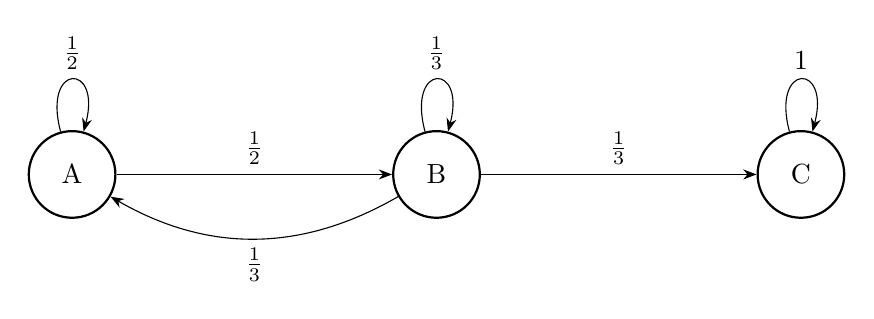
\begin{tikzpicture}[
    >=Stealth,
    node distance=3.5cm,
    state/.style={circle, draw, thick, minimum size=1.1cm, align=center}
]
\node[state] (a) {A};
\node[state, right=of a] (b) {B};
\node[state, right=of b] (c) {C};

\draw[->] (a) to[loop above] node[midway, above] {$\frac{1}{2}$} (a);
\draw[->] (a) -- node[midway, above] {$\frac{1}{2}$} (b);
\draw[->] (b) -- node[midway, above] {$\frac{1}{3}$} (c);
\draw[->] (b) to[loop above] node[midway, above] {$\frac{1}{3}$} (b);
\draw[->] (b) to[bend left=30] node[midway, below] {$\frac{1}{3}$} (a);
\draw[->] (c) to[loop above] node[midway, above] {$1$} (c);
\end{tikzpicture}
\end{document}
